% @out_file dokumentace.tex
% @author Štěpán Faragula
% @brief Dokumentace semestrální práce z předmětu KIV/MBKZ.
% @version 1.0
% @date 2024-05-01

% Document
\documentclass[12pt]{report}

% Čeština
\usepackage[utf8]{inputenc}
\usepackage[T1]{fontenc}
\usepackage[czech]{babel}

% Formát dokumentu
\usepackage{amsmath}
\usepackage{caption}
\usepackage{textcomp}
\usepackage{xspace}
\usepackage{parskip}
\usepackage[hidelinks]{hyperref}

% Graphics
\usepackage{graphicx}
\graphicspath{{img/}}
\usepackage{fancyvrb}
\usepackage[
left=30mm, 
right=30mm, 
top=30mm, 
bottom=30mm,
]{geometry}

% Vychytávky
\usepackage{lipsum}								% Lorem impsum
\usepackage{pdflscape}							% Landscape
\usepackage{menukeys}							% Klavesy
\usepackage{algorithm}							% Algoritmus
\usepackage[noend]{algpseudocode}				% Pseudokod
\usepackage{dirtree}							% Adresarova struktura
												% Tabulky pomoci https://www.tablesgenerator.com/
												

\usepackage{titlesec}
\titleformat{\chapter}{}{\bf\LARGE\thechapter~~~}{0em}{\bf\LARGE}

\newcommand\indentt[1]{						
	\setlength\parindent{5mm}
	#1
	\setlength\parindent{0mm}
}	


% ---------------------	
% Begin
% ---------------------	
\begin{document}


	% ---------------------		
	% Titulní strana
	% ---------------------	
	\begin{titlepage}
		\centering
		\Large
		
		
\includegraphics[width=.7\textwidth]{fav}
		
		\vspace{15mm}
		{\Huge\bfseries Procvičování matematiky}

		\vspace{5mm}
		{\LARGE Katedra informatiky a výpočetní techniky}
		{\LARGE Semestrální práce z předmětu KIV/MBKZ}
		
		\vfill
		\raggedright
		Štěpán Faragula\\
		A21B0119P\\
		farag844@students.zcu.cz
		\hfill 
		\today
	\end{titlepage}

	
	% ---------------------	
	% Obsah
	% ---------------------	
	\tableofcontents


	% ---------------------	
	% Zadání	
	% ---------------------	
	\chapter{Zadání}
	Cílem této semestrální práce je vytvořit aplikaci na procvičování matematiky. Přestože již existují podobné aplikace, zatím se mi nepodařilo najít takovou, která by podporovala počítání se zápornými čísly. Zadání jsem si tedy zvolil vzhledem k osobním potřebám.
	
	Cvičení bude fungovat na jednoduchém principu. Uživateli bude představen náhodně vygenerovaný příklad, ve kterém bude jedna neznámá hodnota. Následně bude muset uhodnout správnou hodnotu, a to buď výběrem ze 4 možností, nebo vlastnoručním vyplněním. Jeden z těchto módů by mohl být pojat ve stylu hry, přičemž se bude navyšovat skóre podle vypočítaných příkladů. 
	
	Při vývoji bude kladen důraz na přizpůsobitelnosti procvičování. Aplikace bude umožňovat měnit volbu rozsahu, ve kterém se mohou čísla vyskytovat, spolu s dalšími možnostmi.



	% ---------------------			
	% Programátorská dokumentace
	% ---------------------	
	\chapter{Programátorská dokumentace}
	Aplikace byla vyvíjena pro platformu Android s úrovní API 24 a vyšší. K tomu bylo použito vývojové prostředí Android Studio.

	Bylo implementováno celkem 5 tříd \texttt{Activity} s vlastním \texttt{ContentView}. Názvy tříd jsou výstižné, ve zkratce se jednotlivé aktivity zabývají následujícím:
	\begin{itemize}
		\item \texttt{Menu} - vstupní bod programu
		\item \texttt{Exercise} - první mód, 4 možné odpovědi
		\item \texttt{Challenge} - druhý mód, ruční zadávání výsledku
		\item \texttt{Settings} - nastavení parametrů
		\item \texttt{About} - stručné informace o aplikaci
	\end{itemize}

	U náhodného generování příkladů se nejprve zvolí matematická operace a jedno náhodné číslo z rozsahu. Další dvě čísla jsou dopočítána. Následně se zvolí, které z čísel by~mělo představovat neznámou hodnotu. V prvním módu se ještě vypočítají 3 nesprávné hodnoty, které jsou také ukázány uživateli.
	
	Nastavení se ukládá do \texttt{SharedPreferences}. Na začátku každého cvičení se přečtou uložená data. V případě kdy neexistují, načtou se výchozí hodnoty.
	
	Aplikace také podporuje zobrazení anglické a české lokalizace spolu s barevným schématem podle uživatelova systému. 

	% ---------------------	
	% Uživatelská dokumentace
	% ---------------------	
	\chapter{Uživatelská dokumentace}
	\section{Hlavní menu}	
	Zobrazí se po spuštění aplikace, slouží k navigaci.
	
	\begin{figure}[ht]
		\centering
		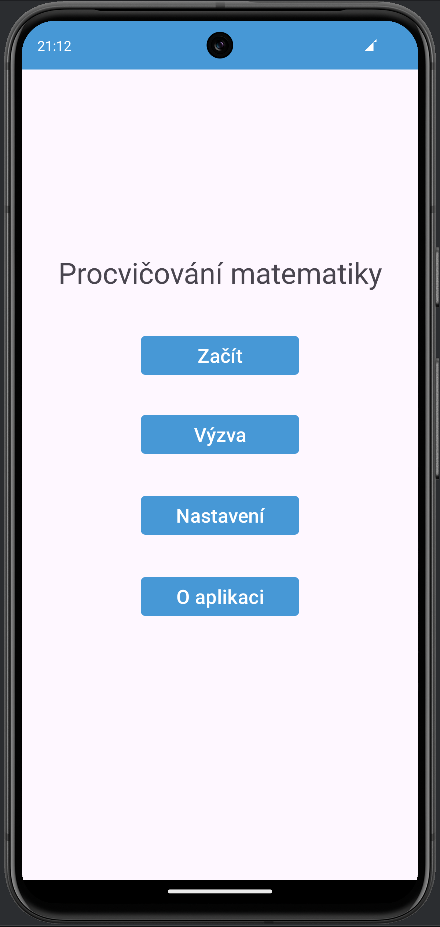
\includegraphics[height=0.9\textwidth]{img/menu}
		\label{fig:menu}
	\end{figure}
	
	\newpage
	\section{Procvičování}
	Uživateli se zobrazí náhodně vygenerovaný příklad spolu se 4 různými možnostmi. Další příklad se zobrazí po vybrání správného výsledku, přičemž se špatné odpovědi podbarví červeně. Na výběr je neomezený čas a po uhodnutí výsledku následuje vteřinová prodleva, která jej zvýrazní. Po určitém počtu příkladů se zobrazí hláška shrnující průběh cvičení. Po stisknutí tlačítka zpět na mobilu se zobrazí dialog, který musí být potvrzen.
	
	\begin{figure}[ht]
		\centering
		\begin{minipage}{.5\textwidth}
			\centering
			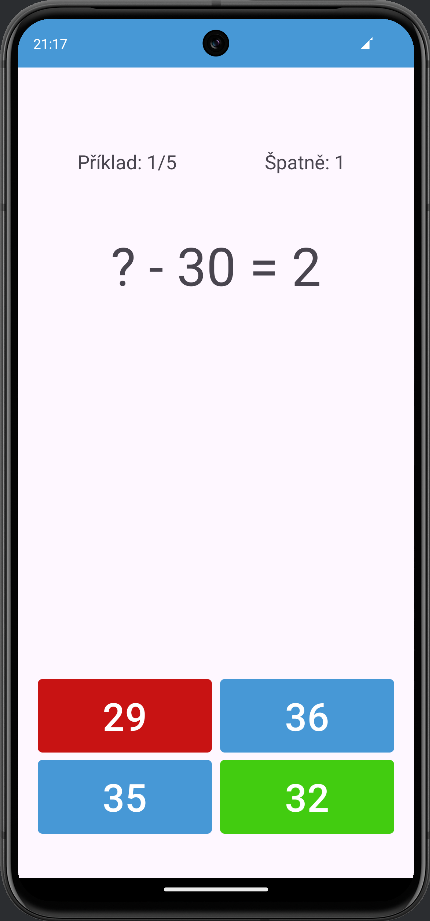
\includegraphics[height=1.7\textwidth]{img/exercise_1}
			\label{fig:exercise_1}
		\end{minipage}%
		\hfill
		\begin{minipage}{.5\textwidth}
			\centering
			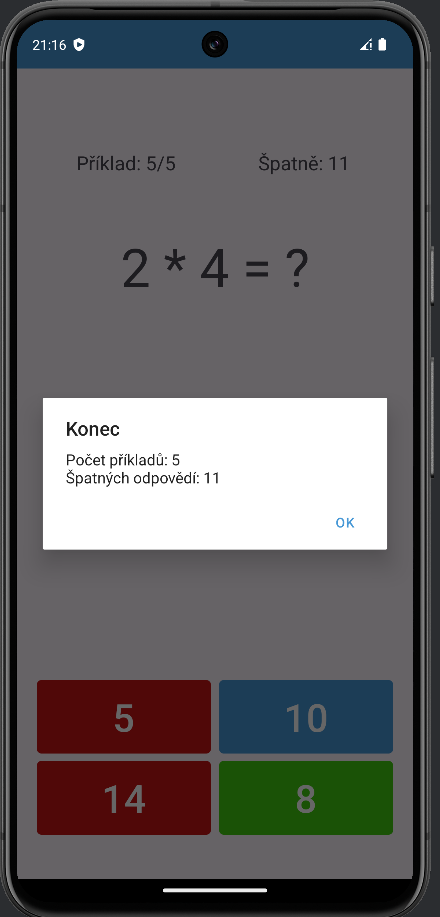
\includegraphics[height=1.7\textwidth]{img/exercise_2}
			\label{fig:exercise_2}
		\end{minipage}
	\end{figure}
	
	\newpage
	\section{Výzva}
	U výzvy musí uživatel zadávat všechny výsledky ručně. Nad příkladem je zobrazeno skóre a jedná se o počet doposud správně vypočítaných příkladů. Jakmile je zadána špatná odpověď, výzva končí. Podle dosaženého skóre je zobrazena jedna z 5 vět, která by měla uživatele dále motivovat.
	
	\begin{figure}[ht]
		\centering
		\begin{minipage}{.5\textwidth}
			\centering
			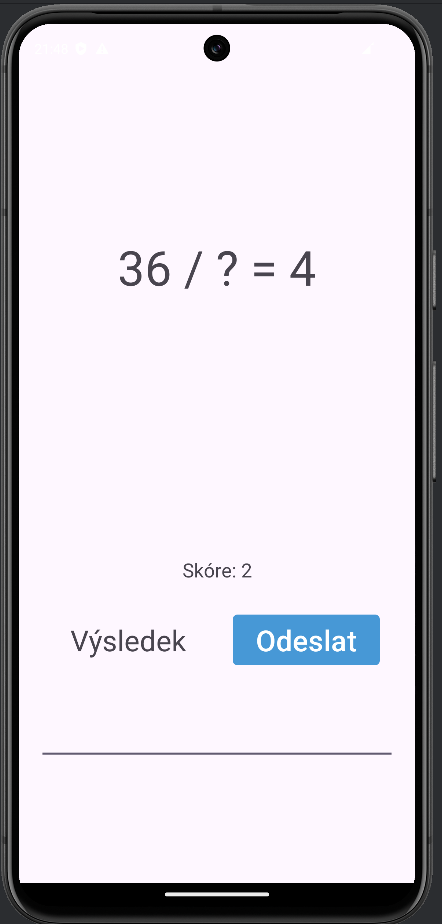
\includegraphics[height=1.7\textwidth]{img/challenge_1}
			\label{fig:challenge_1}
		\end{minipage}%
		\hfill
		\begin{minipage}{.5\textwidth}
			\centering
			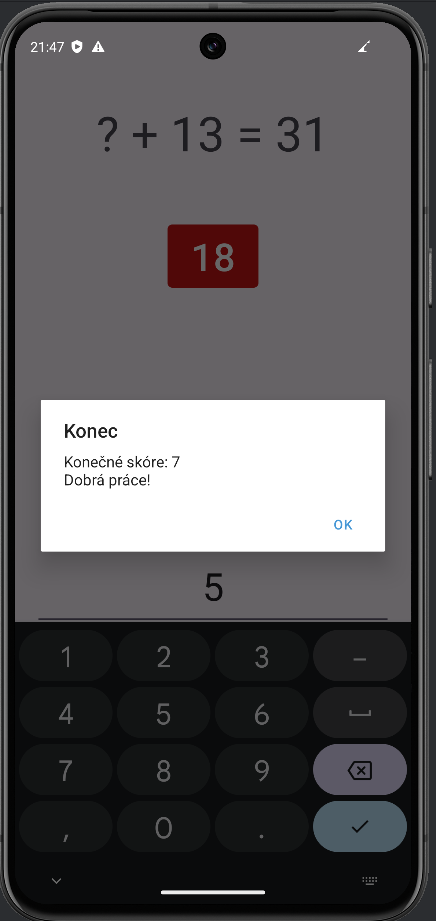
\includegraphics[height=1.7\textwidth]{img/challenge_2}
			\label{fig:challenge_2}
		\end{minipage}
	\end{figure}
	
	\newpage
	\section{Nastavení}
	Aplikace umožňuje měnit průběh cvičení. Provedené změny se budou týkat obou módů, krom počtu příkladů, který se týká pouze prvního. Je možné měnit, na jaké pozici se bude vyskytovat otazník a jaké operace by měly být procvičovány. Rozsah hodnot operací může být i záporný. Dále je možné zvolit tmavý nebo světlý vzhled aplikace, přičemž ve výchozím nastavení je zvolen podle systému Android. Ladící výpis zobrazuje dva příklady, kde v jednom je otazník a ve druhém ne. Všechny možnosti se ukládají pomocí \texttt{SharedPreferences}. Uživatelský vstup je zabezpečen proti neplatným hodnotám.
	
	\begin{figure}[ht]
		\centering
		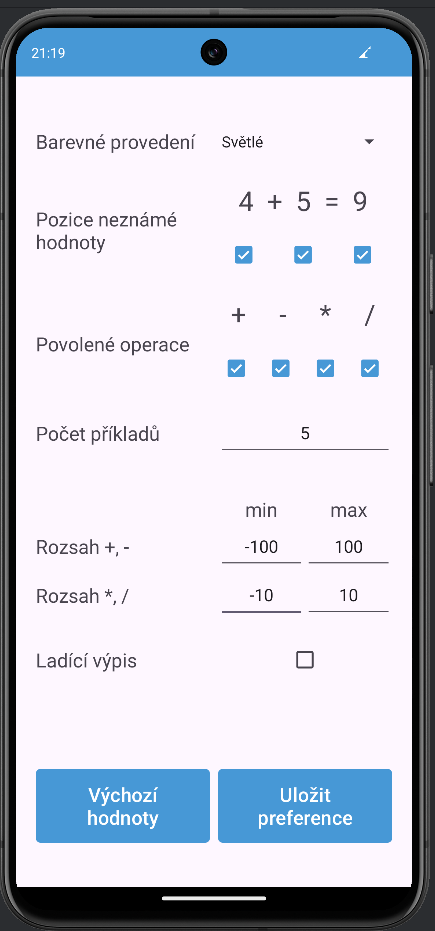
\includegraphics[height=0.9\textwidth]{img/settings}
		\label{fig:settings}
	\end{figure}
	
	\newpage
	\section{O aplikaci}
	Zde jsou vypsány základní informace o aplikaci.
	
	\begin{figure}[ht]
		\centering
		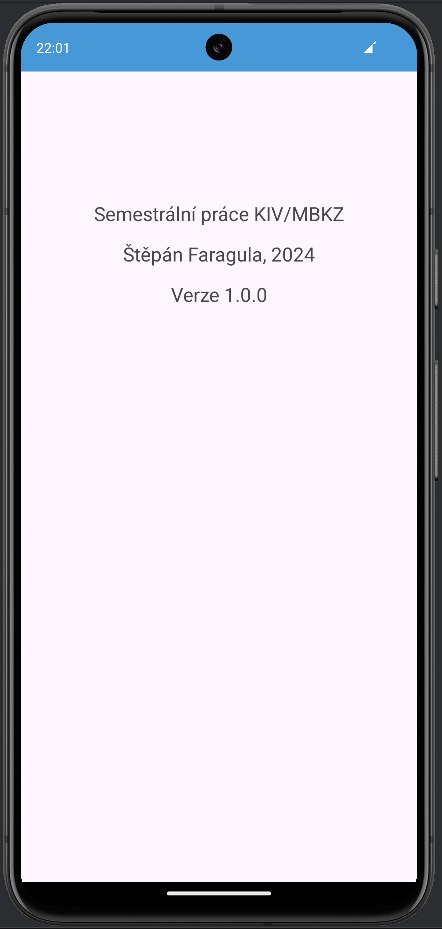
\includegraphics[height=0.9\textwidth]{img/about}
		\label{fig:about}
	\end{figure}
	
	\newpage
	\section{Lokalizace a přenositelnost}
	Uživatelské rozhraní umí přizpůsobit svůj jazyk a barevný motiv podle systému. Momentálně je aplikace přeložena do češtiny a angličtiny. Komponenty jsou adaptivní, dokážou se škálovat podle různých velikostí displejů. Po otočení telefonu se zobrazení nemění. 
	
	\begin{figure}[ht]
		\centering
		\begin{minipage}{.5\textwidth}
			\centering
			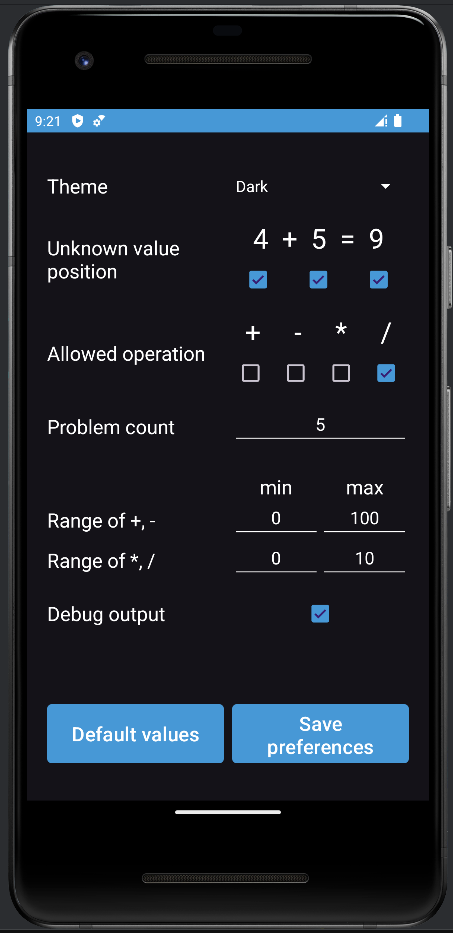
\includegraphics[height=1.7\textwidth]{img/dark_1}
			\label{fig:dark_1}
		\end{minipage}%
		\hfill
		\begin{minipage}{.5\textwidth}
			\centering
			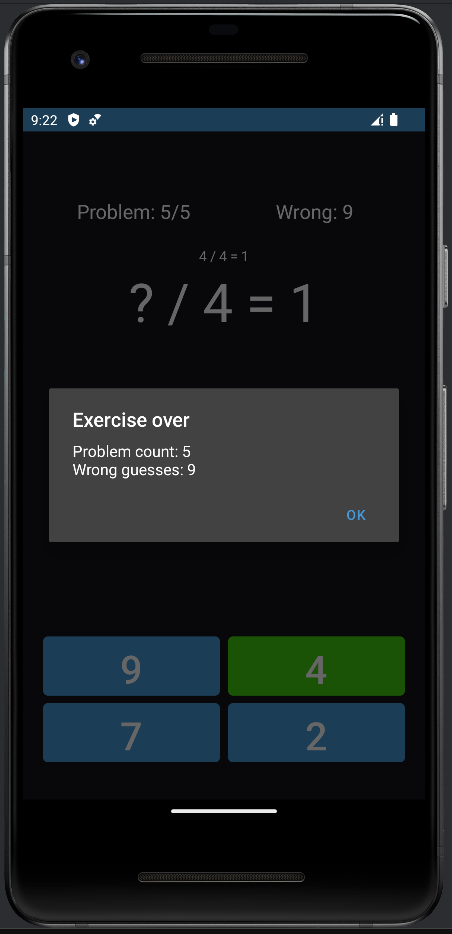
\includegraphics[height=1.7\textwidth]{img/dark_2}
			\label{fig:dark_2}
		\end{minipage}
	\end{figure}


	% ---------------------	
	% Řešené problémy
	% ---------------------	
	\chapter{Řešené problémy}
	Virtuál
	
	Lokalizace podle systému


	% ---------------------	
	% Testování
	% ---------------------	
	\chapter{Testování}
	Pixel 2, Pixel 8
	

	% ---------------------	
	% Závěr
	% ---------------------	
	\chapter{Závěr}
	
	
	
\end{document}
